\section{Modeling of Hypersonic Thermal Protection Systems}

The following discussion presents the modeling of the transient heat conduction problem in multi-layered hypersonic thermal protection systems (TPS) with imperfect contact resistances. Moreover, three different physics-based approaches of decreasing fidelity are presented for solving the governing equations: (i) a fine three-dimensional FEM termed the \emph{full-order model} (FOM), (ii) a one-dimensional FEM with linear elements termed the \emph{one-dimensional FEM} (1D-FEM), and (iii) a lumped-mass representation of the TPS termed the \emph{lumped capacitance model} (LCM). The governing equations and their three solutions strategies are presented next.

\subsection{Governing Equations}

Consider the generic domain $\Omega\subset\mathbb{R}^{d}$ show in Fig.~\ref{fig_general_domain}. A heat flux $q_b$ (i.e., Neumann boundary condition) is prescribed on boundary $e_q$, while a temperature $T_b$ (i.e., Dirichlet boundary condition) is prescribed on boundary $e_T$, and $\partial\Omega = \cup_{i=1}^{N}\partial\Omega_i$ where $e_{iq},e_{iT}\subset\partial\Omega_i$. The transient heat conduction dynamics is governed by the following energy PDE,
\begin{subequations}
 \begin{align}
    \rho c_p \partial_t T - \nabla\cdot\left(\vk(T)\nabla T\right) &= 0, \: x\in\Omega\\
    -\vk(T)\nabla T\cdot\vn &= q_b(x,t), \: x\in e_q\\
    T(x,t) &= T_b(x,t), \: x\in e_T\\
    T(x,0) &= T_0(x), \: x\in\Omega
 \end{align}
\end{subequations}
where the density $\rho$ is constant, while the heat capacity $c_p$ and thermal conductivity $\vk\in\mathbb{R}^{d\times d}$ are temperature-dependent. The TPS domain is divided into $N_C$ non-overlapping components $\left\{\Omega_i\right\}_{i=1}^{N_C}$, where $N_{\Gamma}$ different imperfect contacts are present at the interfaces between components. For example, Fig.~\ref{fig_general_domain} contains $N_C=3$ components and $N_{\Gamma}=3$ imperfect contacts between components. Imperfect contacts translate into \emph{thermal contact resistances} (TCRs), which lead to temperature discontinuities at the interfaces between TPS layers. Therefore, large uncertainties in TCRs may have a significant impact on the overall heat transfer dynamics of TPS. The following discussion presents the simulation of hypersonic TPS under the presence of TCRs, where three different approaches of decreasing fidelity are presented: a full-order three-dimensional finite-element model (FOM), a one-dimensional FEM approximation, and a modified lumped capacitance model (LCM).

\begin{figure}
    \centering
    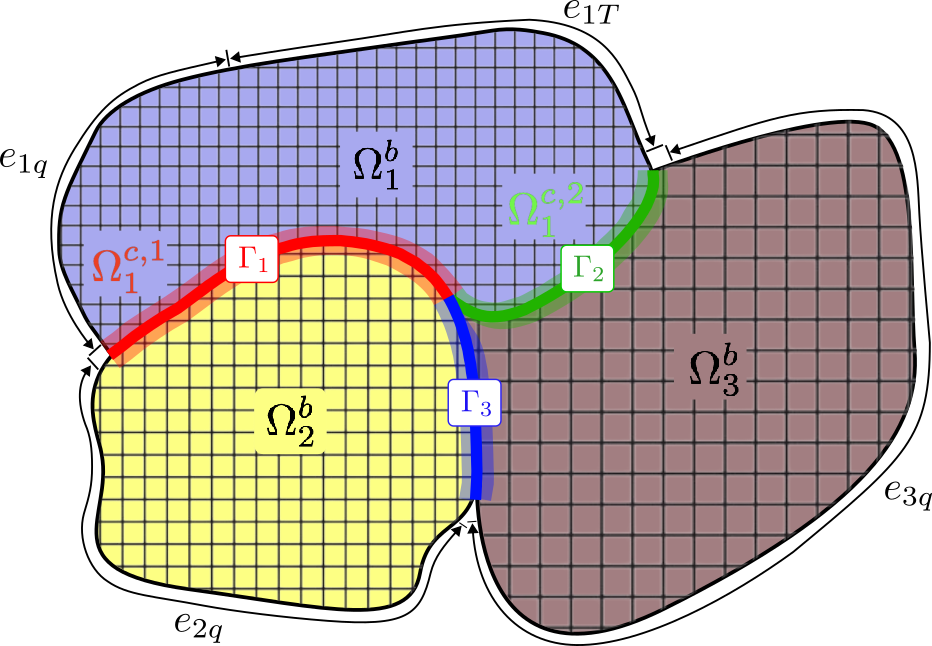
\includegraphics[width=0.99\textwidth]{./figs/modeling/domain.png}
    \caption{Schematic of the general TPS domain $\Omega$ composed of $N_C=3$ components and $N_{\Gamma}=3$ imperfect contacts between components.}
    \label{fig_general_domain}
\end{figure}

\subsection{Full-Order Model}

The FOM is obtained by spatially discretizing the governing PDE using a Discontinuous Galerkin (DG) FEM to result in a high-dimensional system of ordinary differential equations (ODEs) that captures the transient temperature dynamics of the TPS with high fidelity. As in previous work [VargasVenegas2026], the DG-FEM is chosen to describe the FOM as it: (i) provices a systematic framework for modeling multi-layered TPS with complex geometries and material properties, (ii) provides a natural framework for incorporating TCRs at the interfaces, and (iii) is amenable to systematic model reduction via coarse-graining. In Sec. [X] the FOM numerical solutions are performed using standard FEM instead, and the equivalence between DG and standard FEM is noted upon their convergence.

Consider a DG-FEM spatial discretization of the governing PDE, where the entire domain $\Omega$ is partitioned into $M$ non-overlapping elements $\left\{E_i\right\}_{i=1}^M$, where each element belong to one and only one component of the TPS. Moreover, the perfect, imperfect, Neumann, and Dirichlet boundary interfaces are denoted as $e_{ij}$, $\Gamma_{ij}$, $e_{iq}$, and $e_{iT}$, respectively. Lastly, $\left|\partial E_i\right|$ denotes the length $(d=2)$ or area $(d=3)$ of a boundary $\partial E_i$. Now, for the $i$-th element, use a set of $P$ basis functions, such as polynomials, to represent the temperature field as,
\begin{equation}
    T_i(x,t) = \sum_{p=1}^P \vphi_p(x) u_{i,p}(t),\qquad x\in E_i
\end{equation}
Without loss of generality, let the basis functions on element $E_i$ satisfy the following orthogonality condition,
\begin{equation}
    \int_{E_i}\phi_p^i\phi_q^i d\Omega = \left|E_i\right|\delta_{pq},\quad p\neq q\label{eqn_basis_functions_condition}
\end{equation}
where $\delta_{pq}$ is the Kronecker delta. Furthermore, to aid in subsequent model-order reduction derivations, choose $\phi_1^i=1$; therefore, by orthogonality, $\int_{E_i}\phi_p^i d\Omega = 0$ for $p>1$. The first basis function therefore captures the volume-averaged temperature of the element, while the remaining basis functions capture the spatially-varying temperature distributions within the element.

By standard variational procedure, e.g., [Pernet2018], the full governing equation is denoted as,
\begin{equation}
    \vA(\vu)\dot{\vu} = \vB\left(\vu\right)\vu + \vf^{(b)}(t) + \vf^{(c)}(\vu,t)
\end{equation}
where $\vu=\left[\vu_1^\top,\vu_2^\top,\dots,\vu_M^\top\right]^\top\in\mathbb{R}^{MP}$ corresponds to the DG-FEM states, $\vA$ and $\vB$ are the mass and stiffness matrices, respectively, which are functions of the temperature-dependent material properties, and $\vf^{(b)}$ and $\vf^{(c)}$ correspond to the contributions of the boundary conditions and the TCRs, respectively.

\subsection{One-Dimensional Finite-Element Model}

This approach follows a \emph{one-dimensional} FEM (1D-FEM) approach, where the governing PDE is spatially discretized using a standard FEM with linear basis functions along the thickness direction of the TPS, while the in-plane temperature gradients are neglected. This simplification is commonly used in the literature for modeling heat conduction in multi-layered TPS, since under hypersonic thermal loading, the temperature gradient along the thickness direction of the structure is significantly higher than the in-plane temperature gradients, and thus the through-thickness temperature distribution dominates the overall thermal response of the system [Gao2026].

As with the FOM, the TCR introduces additional considerations in the formulation of the 1D-FEM. 

\section{Lumped Capacitance Model with Imperfect Contacts}

This work leverages the \emph{lumped capacitance model} (LCM), a first-principle physics-based model of the TPS that captures the transient component-wise average temperature of the TPS [Incropera2011]. Nonetheless, the presence of TCRs at the interfaces introduces additional modeling considerations since the temperature drop across an interface includes, in addition to the bulk drop across the interface, a contribution from the contact resistance. The following discussion presents the formulation of the LCM for modeling the transient thermal response of the TPS with unknown TCRs, and the separation of dynamics into \emph{bulk} and \emph{contact} contributions.

\paragraph*{Bulk Dynamics} Leveraging our previous work in Ref. [VargasVenegas2026], a modified version of the LCM is leveraged in this work as the physics-based component in the PIROM. The LCM may be derived at the component level from a point of view of energy conservation, and is written as,
\begin{equation}
    \int_{\Omega_i}\rho c_{p,i}(\bar{u})\dot{\bar{u}}_i d\Omega = \sum_{j\in\cN^e_i}\int_{e_{ij}}q^{(e)}_{ij}d\Gamma + \sum_{j\in\cN_i^{c}}\int_{\Gamma_{ij}}q^{(c)}_{ij}d\Gamma + \int_{e_{iq}}q_{b}d\Gamma + \int_{e_{iT}}q_{T}d\Gamma
\end{equation}
where $q^{(e)}_{ij}$ and $q^{(c)}_{ij}$ correspond to the heat flux due to neighboring elements with perfect ($e_{ij}$) and imperfect $(\Gamma_{ij})$ interfacing surfaces, while $q_{ib}$ and $q_{iT}$ are the heat flux contributions from the Neumann and Dirichlet boundary conditions on the $e_{iq}$ and $e_{iT}$ interfaces.



The set $\cN_i$ corresponds to the neighboring components of component $i$, which are defined as those components that share an interface with component $i$. For a perfect contact between components, the heat flux $q_{ij}$ is written as $q_{ij} = G_{ij}(\bar{\vu})(\bar{u}_i - \bar{u}_j)$ where $G_{ij}(\bar{\vu})$ is the effective conductance. However, the presence of TCRs introduces an additional temperature drop across the interface, as discussed next.

\paragraph*{Contact Dynamics} Consider Fig. [X], where the interface $\Gamma_k=\partial\Omega_{l(k)}\cap\partial\Omega_{r(l)}$ is magnified to depict the governing heat transfer mechanisms. For interface $\Gamma_k$ define the average temperature on the 



The variables $\theta_i^-$ and $\theta_i^+$ represent the averaged interfacial temperatures, immediately to the left and to the right of the interface, respectively, while $z_i^-$ and $z_i^+$ represent the thermocouple measurements at distances $\delta_i^-$ and $\delta_i^+$ to the left and right of the interface, respectively. Additionally, $R_i^-$, $R_i^+$, and $R_{x,i}$ correspond to the bulk thermal resistance of the left and right layers, and the contact resistance at the interface, respectively. The total temperature drop across the interface is therefore the sum of the bulk temperature drop and the contact temperature drop, i.e.,
\begin{equation}
    \underbrace{\bar{u}_{i} - \bar{u}_{i+1}}_{\text{total lumped drop}} = \underbrace{\bigl(\bar{u}_i - \theta_i^-\bigr) + \bigl( \theta_i^+  - \bar{u}_{i+1}\bigr)}_{\text{bulk drop}} + \underbrace{\bigl(\theta_i^- - \theta_i^+\bigr)}_{\text{contact drop}}
\end{equation}
hence, the bulk drop becomes,
\begin{equation}
    \left(\bar{u}_i - \theta_i^-\right) + \left( \theta_i^+  - \bar{u}_{i+1}\right) = \left(\bar{u}_i - \bar{u}_{i+1}\right) - \Delta\theta_i 
\end{equation}
Therefore, at an interface $i\in\mathcal{I}$ with a contact resistance, the heat flux between neighboring components may be written as,
\begin{equation}
    q_{ij} = G_{ij}(\bar{\vu})\Bigl(\bigl(\bar{u}_i - \bar{u}_j\bigr) - \Delta\theta_{i}\Bigr)
\end{equation}

\begin{figure}
    \centering
    
\includegraphics[width=0.9\textwidth]{./interface.png}
    \caption{Schematic of the interface between two layers of the TPS, where the temperature drop across the interface is decomposed into a bulk drop and a contact drop.}
    \label{fig_interface}
\end{figure}






Consider the lumped-mass average temperature state,
\begin{equation}
    \vu = \left[u_1, u_2, u_3, u_4\right]^T\in\mathbb{R}^{N}
\end{equation}
and temperature-dependent lumped-capacitance matrix,
\begin{equation}
    A(\vu) = \begin{bmatrix}
        a_1(u_1) & 0 & 0 & 0 \\
        0 & a_2(u_2) & 0 & 0 \\
        0 & 0 & a_3(u_3) & 0 \\
        0 & 0 & 0 & a_4(u_4)
    \end{bmatrix}
\end{equation}
Let the external Neumann forcing be applied to the first lumped mass,
\begin{equation}
    \vf(t) = \begin{bmatrix} f(t) \\ 0 \\ 0 \\ 0 \end{bmatrix}
\end{equation}
For interfaces $i=1,2,3$, define the known \emph{bulk resistances}
\begin{equation}
    S_i(\vu)=R_i^{-}(\vu)+R_i^{+}(\vu)
\end{equation}
and the unknown contact resistance,
\begin{equation}
    R_{xi}>0,\qquad g_{xi}:=\frac{1}{R_{xi}}.
\end{equation}

The classical lumped-capacitance model with effective series resistances is,
\begin{equation}
    A\left(\vu\right)\dot{\vu} = B\left(\vu\right)\vu + \vf(t)\label{eqn_lcm}
\end{equation}
where,
\begin{equation}
    B\left(\vu\right) = \sum_{i=1}^{N-1}\frac{1}{S_i(\vu)+R_{xi}}\vK_i
\end{equation}
with standard nearest-neighbor diffusion stencils,
\begin{equation}
    \vK_1 = \begin{bmatrix}
        1 & -1 & 0 & 0 \\
        -1 & 1 & 0 & 0 \\
        0 & 0 & 0 & 0 \\
        0 & 0 & 0 & 0
    \end{bmatrix},\: \vK_2 = \begin{bmatrix}
        0 & 0 & 0 & 0 \\
        0 & 1 & -1 & 0 \\
        0 & -1 & 1 & 0 \\
        0 & 0 & 0 & 0
    \end{bmatrix},\: \vK_3 = \begin{bmatrix}
        0 & 0 & 0 & 0 \\
        0 & 0 & 0 & 0 \\
        0 & 0 & 1 & -1 \\
        0 & 0 & -1 & 1
    \end{bmatrix}
\end{equation}

The effective heat flux through interface $i$ is therefore,
\begin{equation}
    q_i = \frac{u_{i+1}-u_i}{S_i(\vu)+R_{xi}}
\end{equation}
where the temperature-drop convention is always taken as,
\begin{equation}
    \Delta u_i = u_{i+1}-u_i
\end{equation}

\subsection{Total drop = bulk drop + contact drop}

To separate bulk and contact contributions, introduce interface temperatures
\begin{equation}
    \theta_i^{+},\qquad \theta_i^{-},\qquad i=1,2,3,
\end{equation}
where $\theta_i^{-}$ and $\theta_i^{+}$ are the temperatures immediately to the left and right of contact $i$, respectively. Define the contact temperature jumps as,
\begin{equation}
    \Delta\theta_i:=\theta_i^{+}-\theta_i^{-}, \qquad i=1,2,3
\end{equation}



The total lumped-to-lumped temperature drop across interface $i$,
\begin{equation}
    u_{i+1}-u_i
\end{equation}
This total lumped-to-lumped temperature drop is the sum of the bulk drop across the interface and the contact jump across the interface,
\begin{equation}
    \underbrace{u_{i+1}-u_i}_{\text{total drop}} = \underbrace{\bigl(\theta_i^{-}-u_i\bigr)+\bigl(u_{i+1}-\theta_i^{+}\bigr)}_{\text{bulk drop}} + \underbrace{\bigl(\theta_i^{+}-\theta_i^{-}\bigr)}_{\text{contact drop}}.
\end{equation}
Hence,
\begin{equation}
    \underbrace{\left(\theta_i^- - u_i\right) + \left(u_{i+1}-\theta_i^+\right)}_{\text{bulk drop}} = \underbrace{(u_{i+1}-u_i)}_{\text{total drop}} - \underbrace{\Delta\theta_i}_{\text{contact drop}}
\end{equation}

\begin{equation}
\text{bulk drop across interface }i
=
(u_{i+1}-u_i)-\Delta\theta_i.
\label{eq:bulk_drop}
\end{equation}

Thus the lifted state is
\[
x=
\begin{bmatrix}
u\\ \Deltavtheta
\end{bmatrix}
=
\begin{bmatrix}
u_1\\u_2\\u_3\\u_4\\\Delta\theta_1\\\Delta\theta_2\\\Delta\theta_3
\end{bmatrix}
\in \mathbb{R}^{7},
\qquad
\Deltavtheta=
\begin{bmatrix}
\Delta\theta_1\\\Delta\theta_2\\\Delta\theta_3
\end{bmatrix}.
\]

\subsection{Heat-flux Continuity and DAE Formulation}

Using the adopted convention, define the bulk and contact heat fluxes as
\begin{equation}
q_i^{(b)}
=
\frac{(u_{i+1}-u_i)-\Delta\theta_i}{S_i(u)},
\qquad
q_i^{(c)}
=
\frac{\Delta\theta_i}{R_{xi}}
=
g_{xi}\Delta\theta_i.
\label{eq:q_bulk_contact}
\end{equation}

Heat-flux continuity across each interface requires
\begin{equation}
q_i^{(b)}=q_i^{(c)},
\qquad i=1,2,3,
\label{eq:flux_continuity}
\end{equation}
which yields the algebraic constraints
\begin{equation}
\frac{(u_{i+1}-u_i)-\Delta\theta_i}{S_i(u)}
-
g_{xi}\Delta\theta_i
=
0,
\qquad i=1,2,3.
\label{eq:algebraic_constraints}
\end{equation}

\subsection*{Lumped-temperature dynamics}

The four lumped energy balances yield,
\begin{subequations}
    \begin{align}
        a_1(u_1)\dot u_1 &= f(t) - q_{12}^{(b)}\\
        a_2(u_2)\dot u_2 &= q_{12}^{(b)} - q_{23}^{(b)}\\
        a_3(u_3)\dot u_3 &= q_{23}^{(b)} - q_{34}^{(b)}\\
        a_4(u_4)\dot u_4 &= q_{34}^{(b)}
    \end{align}
\end{subequations}
Substituting using the bulk heat fluxes yields,
\begin{subequations}
    \begin{align}
        a_1(u_1)\dot u_1 &= f(t) - \frac{(u_2-u_1)-\Delta\theta_1}{S_1(u)}\\
        a_2(u_2)\dot u_2 &= \frac{(u_2-u_1)-\Delta\theta_1}{S_1(u)} - \frac{(u_3-u_2)-\Delta\theta_2}{S_2(u)}\\
        a_3(u_3)\dot u_3 &= \frac{(u_3-u_2)-\Delta\theta_2}{S_2(u)} - \frac{(u_4-u_3)-\Delta\theta_3}{S_3(u)}\\
        a_4(u_4)\dot u_4 &= \frac{(u_4-u_3)-\Delta\theta_3}{S_3(u)}
    \end{align}
\end{subequations}

\subsection*{Matrix form of DAE}

Define the difference matrix,
\begin{equation}
    \vD = \begin{bmatrix}
    -1 & 1 & 0 & 0 \\
    0 & -1 & 1 & 0 \\
    0 & 0 & -1 & 1
    \end{bmatrix}, \:
    \vD u = \begin{bmatrix}
    u_2-u_1 \\
    u_3-u_2 \\
    u_4-u_3
    \end{bmatrix}
\end{equation}
Define the bulk temperature stencils,
\begin{equation}
    \vK_1 = \begin{bmatrix}
        1 & -1 & 0 & 0 \\
        -1 & 1 & 0 & 0 \\
        0 & 0 & 0 & 0 \\
        0 & 0 & 0 & 0
    \end{bmatrix},\: \vK_2 = \begin{bmatrix}
        0 & 0 & 0 & 0 \\
        0 & 1 & -1 & 0 \\
        0 & -1 & 1 & 0 \\
        0 & 0 & 0 & 0
    \end{bmatrix},\: \vK_3 = \begin{bmatrix}
        0 & 0 & 0 & 0 \\
        0 & 0 & 0 & 0 \\
        0 & 0 & 1 & -1 \\
        0 & 0 & -1 & 1
    \end{bmatrix}
\end{equation}
and the bulk jump-coupling stencils,
\begin{equation}
    \vL_1 = \begin{bmatrix}
        1 & 0 & 0 \\
        -1 & 0 & 0 \\
        0 & 0 & 0 \\
        0 & 0 & 0
    \end{bmatrix},\: \vL_2 = \begin{bmatrix}
        0 & 0 & 0 \\
        0 & 1 & 0 \\
        0 & -1 & 0 \\
        0 & 0 & 0
    \end{bmatrix},\: \vL_3 = \begin{bmatrix}
        0 & 0 & 0 \\ 
        0 & 0 & 0 \\
        0 & 0 & 1 \\
        0 & 0 & -1
    \end{bmatrix}
\end{equation}
Then,
\begin{equation}
    A(u)\dot{u} = \sum_{i=1}^{N-1}\frac{1}{S_i(u)}\Bigl(\vK_i u+\vL_i\Deltavtheta\Bigr) + \vf(t)
\end{equation}
and the algebraic constraints for heat flux continuity are written as,
\begin{equation}
    \operatorname{diag}\!\left(\frac{1}{S_1(u)},\frac{1}{S_2(u)},\frac{1}{S_3(u)}\right)\vD u - \left[\operatorname{diag}\!\left(\frac{1}{S_1(u)},\frac{1}{S_2(u)},\frac{1}{S_3(u)}\right) + G_x\right]\Deltavtheta = 0\label{eqn_algebraic_heat_flux_constraints}
\end{equation}
where
\begin{equation}
    G_x = \begin{bmatrix}
    g_{x1} & 0 & 0 \\
    0 & g_{x2} & 0 \\
    0 & 0 & g_{x3}
    \end{bmatrix}
\end{equation}
Equation \eqref{eqn_algebraic_heat_flux_constraints}, along with the lumped-temperature dynamics, defines a DAE system for the lifted state $x=[u,\Deltavtheta]$.

\subsection{DAE index reduction}

The DAE is index-reduced by differentiating the heat-flux continuity constraints with respect to time, which, for each interface $i$, yields,
\begin{equation}
    \frac{d}{dt}\left[\frac{(u_{i+1}-u_i)-\Delta\theta_i}{S_i(u)} - g_{xi}\Delta\theta_i\right] = 0
\end{equation}
The contact conductances $g_{xi}$ are assumed constant, therefore,
\begin{equation}
    \bigl(1+g_{xi}S_i(u)\bigr)\Delta\dot{\theta}_i = \bigl(\dot{u}_{i+1} - \dot{u}_i\bigr) - \frac{(u_{i+1}-u_i)-\Delta\theta_i}{S_i(u)}\dot{S}_i(u)
\end{equation}
Using the original algebraic constraint
\begin{equation}
    \frac{(u_{i+1}-u_i)-\Delta\theta_i}{S_i(u)}=g_{xi}\Delta\theta_i,    
\end{equation}
the index-reduced dynamics become,
\begin{equation}
    \boxed{
    \Delta\dot{\theta}_i = \frac{ \dot{u}_{i+1}-\dot{u}_i - g_{xi}\Delta\theta_i\,\dot{S}_i(u)}{1+g_{xi}S_i(u)}, \qquad i=1,2,3}
\end{equation}

Define
\begin{equation}
    M(u;R_x) = \begin{bmatrix}
        1+g_{x1}S_1(u) & 0 & 0 \\
        0 & 1+g_{x2}S_2(u) & 0 \\
        0 & 0 & 1+g_{x3}S_3(u)
    \end{bmatrix}
\end{equation}
and,
\begin{equation}
    \dot{S}(u) = \begin{bmatrix}
        \dot{S}_1(u) \\
        \dot{S}_2(u) \\
        \dot{S}_3(u)
    \end{bmatrix},\qquad \Deltavtheta\odot \dot{S}(u) = \begin{bmatrix}
    \Delta\theta_1\dot{S}_1(u) \\
    \Delta\theta_2\dot{S}_2(u) \\
    \Delta\theta_3\dot{S}_3(u)
    \end{bmatrix}
\end{equation}
Then, the index-reduced dynamics for the contact jumps can be written in matrix form as,
\begin{equation}
    M(u;R_x)\Delta\dot{\theta} = D\,\dot u - G_x\bigl(\Deltavtheta\odot \dot S(u)\bigr)
\end{equation}
Thus, the index-reduced lifted system is given by the coupled ODEs,
\begin{subequations}
    \begin{align}
        A(u)\dot{u} &= \sum_{i=1}^{N-1}\frac{1}{S_i(u)}\Bigl(\vK_i u + \vL_i\Deltavtheta\Bigr) + \vf(t)\\
        M(u;R_x)\Delta\dot{\theta} &= \vD\dot{u} - G_x\bigl(\Deltavtheta\odot \dot S(u)\bigr)
    \end{align}
\end{subequations}
